\chapter{实验一:梯度下降单机优化}\label{chapter:task1}

\section{实验内容与要点介绍}

\subsection{实验内容与要求}

\subsubsection{实验内容}
\begin{itemize}
    \item 了解常用优化算法:梯度下降、牛顿法等;
    \item 编写相应的算法实现代码,并进行实验;
    \item 分析一阶方法和二阶方法的实验结果;
    \item 分析确定性算法和随机性算法实验结果。
\end{itemize}
% \item 了解优化器的作用与构建方式(以PyTorch为例)
% \item 构建一阶确定性、一阶随机性优化算法,实现GD、SGD、Adam优化算法
% \item 分析确定性优化算法与随机性优化算法实验结果

\subsubsection{实验要求}
\begin{itemize}
    \item 在MNIST数据集上完成图像分类任务
    \item 实现GD、SGD、ADAM三种基于梯度的优化方法, 写出三个优化器类
    \item 绘制三种优化方法下的loss函数变化图像,通过loss图像及其他实验结果,分析三种优化方法的特点
\end{itemize}

\subsection{PyTorch优化器}

\subsubsection{优化器是干什么用的}

下面展示了一段简单的网络训练过程的代码,我们通过这段代码来理解PyTorch中优化器所发挥的作用。

\begin{lstlisting}
def train_loop(dataloader, model, loss_fn, optimizer):
    size = len(dataloader.dataset)
    for batch, (X, y) in enumerate(dataloader):
        # Compute prediction and loss
        pred = model(X)
        loss = loss_fn(pred, y)
        
        # Backpropagation
        optimizer.zero_grad()
        loss.backward()
        optimizer.step()
\end{lstlisting}
    
在这段代码中\graylstinline{model}为神经网络模型,通过\graylstinline{model(X)}调用了\graylstinline{model}中的\graylstinline{forward}方法,即进行正向传播,获得神经网络输出(第5行)。然后通过损失函数\graylstinline{loss_fn}计算神经网络输出\graylstinline{pred}与数据真实值或标签\graylstinline{y}的差距得到损失值\graylstinline{loss}(第6行)。
得到损失值后,通过反向传播(第10行),网络\graylstinline{model}中的各个参数对应的梯度将会得到更新,得到各个参数的梯度后,优化器\graylstinline{optimizer}便可以根据既定的优化算法来更新参数(第11行)。需要注意的是,神经网络的梯度参数并不是储存最近一次反向传播(即调用\graylstinline{loss.backward()})的结果,而是会将反向传播得到的梯度与当前储存的值相加。因此,我们需要第9行\graylstinline{optimizer.zero_grad()}来将神经网络\graylstinline{model}中储存的梯度值置为0。

如果你是第一次看到类似代码,你可能还会疑惑上述代码中优化器\graylstinline{optimizer}和\graylstinline{model}似乎并没有建立联系,那为什么优化器能处理\graylstinline{model}中的参数呢?这是因为在这个函数之外,\graylstinline{model}中的参数\graylstinline{model.parameters()}早就被喂给\graylstinline{optimizer}了:
\begin{lstlisting}
    optimizer = torch.optim.SGD(model.parameters(), lr=learning_rate)
\end{lstlisting}

\subsubsection{如何在优化器中实现自己的算法}

从上面的例子中可以看到,除了构建函数外,一个最简单的优化器只需要实现\graylstinline{zero_grad}和\graylstinline{step}方法即可。此处需要注意的有这几点:
\begin{itemize}
    \item 当我们手动更改\graphicspath{model}中参数或梯度的值时候,需要将其从计算图中分离。即在\graylstinline{zero_grad}方法中,应包含\graylstinline{param.grad.detach_()}。
    \item 使用Adam算法时,由于还需要上一步优化得到的状态,因此可在初始化函数中构建一个字典用来储存状态。
\end{itemize}

\subsection{MindSpore优化器}

除了使用Pytorch,我们还鼓励同学们使用MindSpore来完成实验。

在MindSpore中,可以通过继承\graylstinline{mindspore.nn.optim.optimizer.Optimizer}类来自定义自己的优化器。在Pytorch中,我们需要实现构造函数和\graylstinline{step()}函数,类似的,在MindSpore中,我们需要实现构造函数和\graylstinline{construct()}函数,\graylstinline{construct()}函数与\graylstinline{step()}函数作用类似。

在构造函数中,我们将神经网络参数、学习速率、衰减速率等变量存入实例。而与Pytorch的\graylstinline{step()}函数不同的是,\graylstinline{construct()}函数需要\graylstinline{gradients}参数作为输入。并且在计算完新的神经网络参数值后,需要使用\graylstinline{mindspore.ops.assign(old_param, new_param)}函数将新的参数值赋予神经网络。

一个简单的优化器实现如下:
\begin{lstlisting}
    from mindspore.nn.optim.optimizer import Optimizer
    from mindspore import ops

    class GdOptimizer(Optimizer):
        def __init__(self, params, lr=0.001):
            super(GdOptimizer, self).__init__(lr, params)

        
        def construct(self, gradients):
            success = None
            for param, grad in zip(self.parameters, gradients):
                update = param - self.learning_rate * grad
                success = ops.assign(param, update)
            return success
\end{lstlisting}

更多资料还可以参考mindspore官方文档:\url{https://mindspore.cn/tutorials/zh-CN/r2.0.0-alpha/advanced/modules/optimizer.html?highlight=%E8%87%AA%E5%AE%9A%E4%B9%89%E4%BC%98%E5%8C%96%E5%99%A8}

\subsection{几种算法回顾}

梯度下降 Gradient Descent:
\begin{align} 
w_{t+1} = w_t - \eta \nabla f(w_t)
\end{align}
随机梯度下降 Stochastic gradient descent:
\begin{align} 
w_{t+1} = w_t - \eta \nabla f_i(w_t)
\end{align}
Adam:
\begin{align} % amsmath package
    m_{t+1} & = \beta_1 m_t + (1-\beta_1) \nabla f(w_t)   \\
    g_{t+1} & = \beta_2 g_t + (1-\beta_2) (\nabla f(w_t))^2
\end{align}


\section{使用VSCode与本地环境调试运行}\label{sec:task1-local-debug}

如果你已经完成了本地环境配置(\S\ref{sec:local-env}),那就可以打开VSCode进行下面的操作了:

\begin{enumerate}
    \item 安装Python插件,如图\ref{fig:task1-vscode-extension-install-python}所示。
        \begin{figure}[htbp]
            \centering
            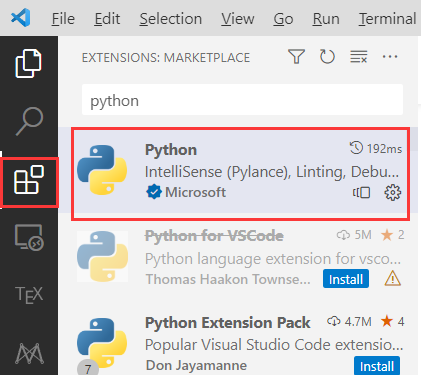
\includegraphics[width=0.7\textwidth]{figures/task1-vscode-extension-install-python.png}
            \caption{caption:task1-vscode-extension-install-python}
            \label{fig:task1-vscode-extension-install-python}
        \end{figure}
    \item 选择Python解释器,按下\graylstinline{F1}或\graylstinline{Ctrl}+\graylstinline{Shift}+\graylstinline{P},输入 "select interpreter"并选择 “Python: Select Interpreter”项(图\ref{fig:task1-vscode-local-select-interpreter})。然后选择:select at work space level。最后选择你在\S\ref{subsec:local-env-create}一孝节中创建的环境对应的解释器(图\ref{fig:task1-vscode-local-select-my-env}中为助教自己创建的distributedml环境)。
        \begin{figure}[htbp]
            \centering
            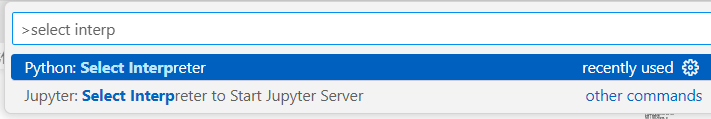
\includegraphics[width=0.7\textwidth]{figures/task1-vscode-local-select-interpreter.png}
            \caption{caption:task1-vscode-local-select-interpreter}
            \label{fig:task1-vscode-local-select-interpreter}
        \end{figure}
        \begin{figure}[htbp]
            \centering
            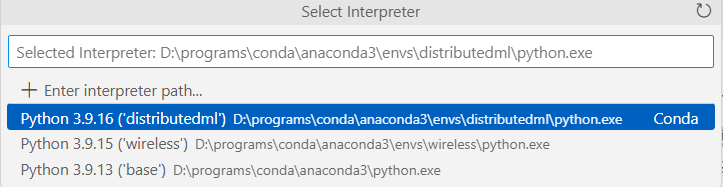
\includegraphics[width=0.7\textwidth]{figures/task1-vscode-local-select-my-env.png}
            \caption{caption:task1-vscode-local-select-my-env}
            \label{fig:task1-vscode-local-select-my-env}
        \end{figure}
    \item 最后,打开自己的.py文件,可以在编辑器右上角看到一个播放形状的三角,点击它或在下拉列表中选择运行或调试,即可开始运行或调试啦。
    \begin{figure}[htbp]
        \centering
        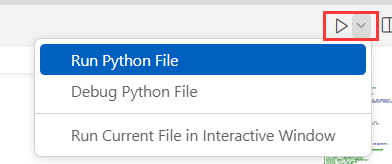
\includegraphics[width=0.5\textwidth]{figures/task1-vscode-local-run-or-debug.png}
        \caption{caption:task1-vscode-local-run-or-debug}
        \label{fig:task1-vscode-local-run-or-debug}
    \end{figure}
\end{enumerate}


\section{使用VSCode与本地容器调试运行}\label{sec:vscode-and-docker-container}

\subsection{启动容器并挂载本地文件夹}\label{subsec:docker-run-and-mount-volume}

在\S\ref{subsec:container-to-image}一小节中,我们创建了自己的镜像,现在,我们需要先启动这个镜像(对于助教而言是\graylstinline{cantjie/pytorch:1.13.1})。但是,目前镜像里面可没有我们写好的代码,而且,就算我们在镜像里面写好代码,该怎么拿出来交作业呢?

为了解决这个问题,我们就需要将本地的目录挂载到容器上,在启动容器时,我们使用\graylstinline{-v <host-dir>:<container-dir>}参数,参考下面命令执行:
\begin{lstlisting}
    $ docker run -it --gpus all -v $pwd/relative/path/to/code:/workspace cantjie/pytorch:1.13.1
\end{lstlisting}

现在进入容器后,我们可以看到,如图\ref{fig:task1-docker-run-with-mount}所示,本地的代码已经被挂载到了\graylstinline{\workspace}文件夹下。
\begin{figure}[htbp]
	\centering
	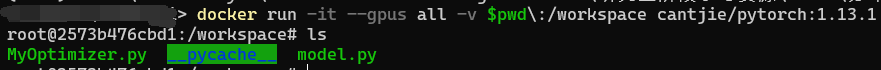
\includegraphics[width=0.9\textwidth]{figures/task1-docker-run-with-mount.png}
	\caption{caption:task1-docker-run-with-mount}
	\label{fig:task1-docker-run-with-mount}
\end{figure}

\subsection{在VSCode中使用容器}

首先安装Dev Container插件,然后按下\graylstinline{Ctrl}+\graylstinline{Shift}+\graylstinline{P},并找到Attatch to Running Container命令,如图\ref{fig:task1-vscode-attach-to-container-quick-search}。
\begin{figure}[htbp]
	\centering
	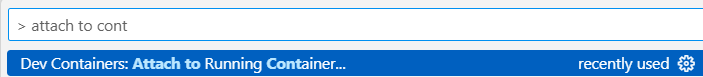
\includegraphics[width=0.7\textwidth]{figures/task1-vscode-attach-to-container-quick-search.png}
	\caption{caption:task1-vscode-attach-to-container-quick-search}
	\label{fig:task1-vscode-attach-to-container-quick-search}
\end{figure}

接下来会弹出一个新窗口,在这个新窗口中,就像在本地环境下调试运行一样在容器里调试运行即可。余下的步骤基本参考上一小节\S\ref{sec:task1-local-debug}中的操作即可。即
\begin{itemize}
    \item 在VSCode侧边栏Explorer栏目中打开\graylstinline{/workspace}目录。
    \item 在VSCode安装Python插件。
    \item 选择编译器为\graylstinline{/opt/conda/bin/python}
\end{itemize}

\section{使用VSCode与远程服务器调试运行}

% 深研院平台和华为云平台的远程服务器使用方法类似,此处以学校的环境为例。
\subsection{使用深研院计算资源}\label{subsec:task1-vscode-using-sigs-resources}
在学校的计算平台创建了开发环境后,平台会提供ssh链接地址以及用户名和密码,我们使用该信息链接远程环境。

首先在VSCode中安装Remote SSH插件,然后按下\graylstinline{Ctrl}+\graylstinline{Shift}+\graylstinline{P},搜索Remote-SSH: Open SSH Configuration File命令(图\ref{fig:task1-open-ssh-config-file})。
\begin{figure}[htbp]
	\centering
	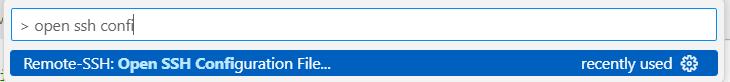
\includegraphics[width=0.7\textwidth]{figures/task1-open-ssh-config-file.png}
	\caption{caption:task1-open-ssh-config-file}
	\label{fig:task1-open-ssh-config-file}
\end{figure}

在下拉列表中选择 C:\textbackslash Users\textbackslash <username>\textbackslash .ssh.

\begin{figure}[htbp]
	\centering
	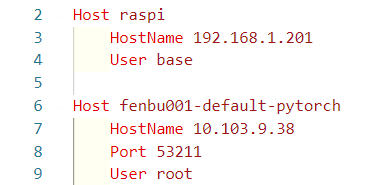
\includegraphics[width=0.6\textwidth]{figures/task1-ssh-config-file-demo.png}
	\caption{ssh config file demo。注意,图中示例包含两个主机。}
	\label{fig:task1-ssh-config-file-demo}
\end{figure}

在打开的.ssh文件中, 按照图\ref*{fig:task1-ssh-config-file-demo}给出的格式,添加一个主机。其中Host对应昵称,HostName为远程主机IP。

\begin{figure}[htbp]
	\centering
	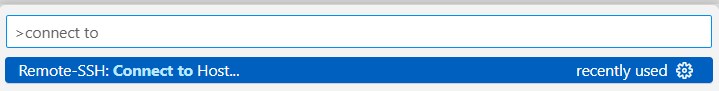
\includegraphics[width=0.7\textwidth]{figures/task1-vscode-connect-to-host-quick-search.png}
	\caption{caption:task1-vscode-connect-to-host-quick-search}
	\label{fig:task1-vscode-connect-to-host-quick-search}
\end{figure}

最后,\graylstinline{Ctrl}+\graylstinline{Shift}+\graylstinline{P}并搜索Remote-SSH: Connect to Host命令,并在后续选择刚刚创建的主机信息。

\begin{figure}[htbp]
	\centering
	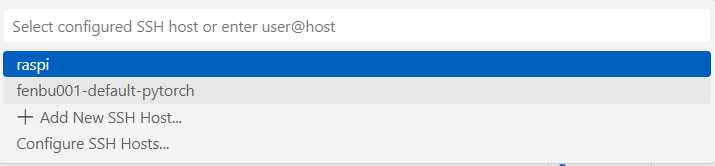
\includegraphics[width=0.7\textwidth]{figures/taks1-vscode-connect-to-certain-host-quick-search.png}
	\caption{caption:taks1-vscode-connect-to-certain-host-quick-search}
	\label{fig:taks1-vscode-connect-to-certain-host-quick-search}
\end{figure}

在弹出的窗口等待连接,并输入密码。余下的步骤又和上一小节\S\ref{sec:vscode-and-docker-container}一样了:打开文件夹、安装Python扩展、指定解释器。此处不再赘述。

\subsection{使用华为云计算资源}

\subsubsection{手动配置}

同使用深研院计算资源\S\ref{subsec:task1-vscode-using-sigs-resources}一样,我们也通过编辑C:\textbackslash Users\textbackslash <username>\textbackslash .ssh中的config文件,来配置ssh链接。在配置前,首先进入华为云的开发环境实例中查看实例的ssh地址,如图\ref{fig:task1-huawei-modelarts-ssh-address}所示,该实例对应的用户名、地址和端口分别为\graylstinline{ma-user}、\graylstinline{dev-modelarts-cnnorth4.huaweicloud.com}、\graylstinline{30194}。

\begin{figure}[htbp]
	\centering
	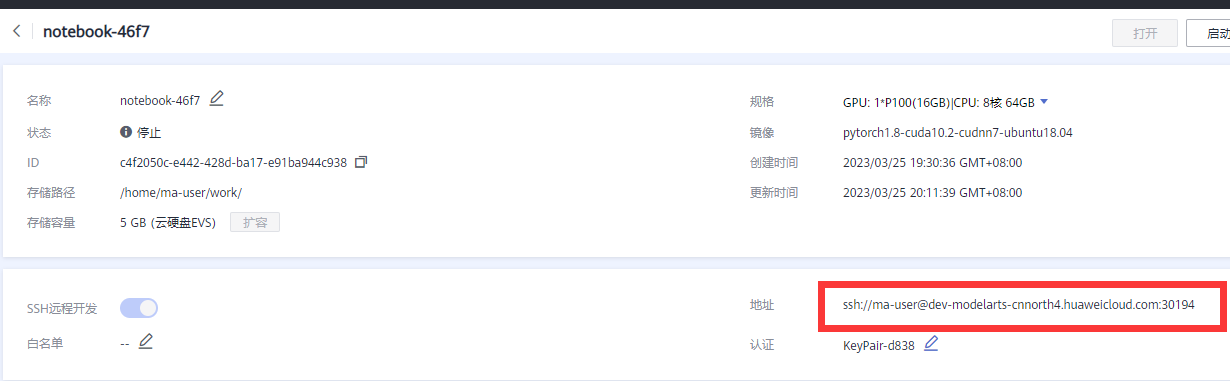
\includegraphics[width=0.9\textwidth]{figures/task1-huawei-modelarts-ssh-address.png}
	\caption{caption:task1-huawei-modelarts-ssh-address}
	\label{fig:task1-huawei-modelarts-ssh-address}
\end{figure}


打开config文件,在原来的基础上加入如图\ref{fig:task1-huawei-modelarts-ssh-config-demo}所示内容。注意根据你的实例和秘钥对修改其中HostName、Port、User、IdentityFile字段。

\begin{figure}[htbp]
	\centering
	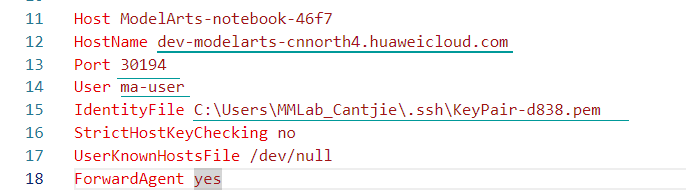
\includegraphics[width=0.8\textwidth]{figures/task1-huawei-modelarts-ssh-config-demo.png}
	\caption{caption:task1-huawei-modelarts-ssh-config-demo}
	\label{fig:task1-huawei-modelarts-ssh-config-demo}
\end{figure}

然后又和上一节一样了,用Remote-SSH插件的Connect to Host命令接入该实例即可。

\subsubsection{使用ModelArts插件自动配置}

聪明的你可能已经发现不同于深研院的平台,华为ModelArts平台中,开发环境实例最右侧操作的更多选项里有一个VS Code接入选项,图\ref{fig:task1-huawei-modelarts-vscode-auto-connect}。如果我们已经安装了VS Code的Remote-SSH插件,我们直接点击“VS Code接入”就可以开始远程开发了。
\begin{figure}[htbp]
	\centering
	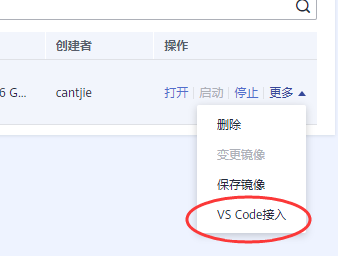
\includegraphics[width=0.4\textwidth]{figures/task1-huawei-modelarts-vscode-auto-connect.png}
	\caption{caption:task1-huawei-modelarts-vscode-auto-connect}
	\label{fig:task1-huawei-modelarts-vscode-auto-connect}
\end{figure}

第一次点击的时候,可能会提示你没有安装一个ModelArts-HuaweiCloud插件,如图\ref{fig:task1-huawei-modelarts-vscode-auto-connect-extension-error},我们点击Install and Open即可。




\begin{figure}[htbp]
	\centering
	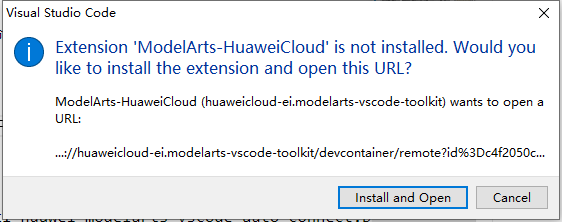
\includegraphics[width=0.6\textwidth]{figures/task1-huawei-modelarts-vscode-auto-connect-extension-error.png}
	\caption{caption:task1-huawei-modelarts-vscode-auto-connect-extension-error}
	\label{fig:task1-huawei-modelarts-vscode-auto-connect-extension-error}
\end{figure}

这时如果你打开C:\textbackslash Users\textbackslash <username>\textbackslash .ssh\textbackslash config文件,你会发现刚刚安装的插件的作用其实就是帮你自动写入图\ref{fig:task1-huawei-modelarts-ssh-config-demo}中的内容。


\subsection{使用密钥对登录远程服务器(可选)}

在使用深研院计算资源和docker容器的时候,你可能已经发现,每次登录都要输入密码,有点麻烦。我们现在可以使用密钥对来实现免密登录远程服务器或容器。

具体而言,在本地(以助教的windows为例),打开终端,使用\graylstinline{ssh-keygen}命令,生成一对秘钥对:
\begin{lstlisting}
    ssh-keygen -t ed25519
\end{lstlisting}
然后在提示下按下三次回车,当然你也可以选择自定义这些内容,不过一般使用默认的设置和空的passphrase就可以了。


我们按照第一次按回车时提示的目录,找到这对密钥对,对于windows,一般是在:
C:\textbackslash Users \textbackslash <username>\textbackslash .ssh目录下的\graylstinline{id_ed25519}私钥文件和\graylstinline{id_ed25519.pub}的公钥文件。

接下来我们需要将公钥文件发送给服务器或容器。如果你的终端可以运行\graylstinline{ssh-copy-id}命令,那么你只需要在终端运行下面的命令即可将公钥发送。
\begin{lstlisting}
    ssh-copy-id user@serverip
\end{lstlisting}

然而,如果你的终端找不到\graylstinline{ssh-copy-id}命令,那么发送过程会稍微麻烦一些:手动将公钥内容写入服务器的\graylstinline{\~/.ssh/authorized_keys}文件中:
\begin{lstlisting}
    # first ssh into the server or container
    # copy the content of your <id_ed25519.pub> into <authorized_keys>
    vi \~/.ssh/authorized_keys
    
    # give the <authorized_keys> propoer permissions
    chmod 600 ~/.ssh/authorized_keys    
\end{lstlisting}
这样就完成公钥的发送了。之后你从终端ssh到服务器,就不再需要密码了。


\subsubsection{可能的问题:权限错误}

如果你在ssh时遇到了权限错误的提示,那很可能是你的本地的私钥的权限出问题了。找你的私钥文件,右键查看属性,在<安全>标签页点击编辑。如果你发现<组或用户名>栏目中有多个项目,如图\ref{fig:task1-ssh-private-key-permission-in-windows}所示(其中马赛克挡住的应该是你目前登录的用户),那么你需要将除了你自己之外的其他用户都删掉,变成图\ref{fig:task1-ssh-private-key-right-permission-in-windows}所示的那样。

\begin{figure}[htbp]
	\centering
	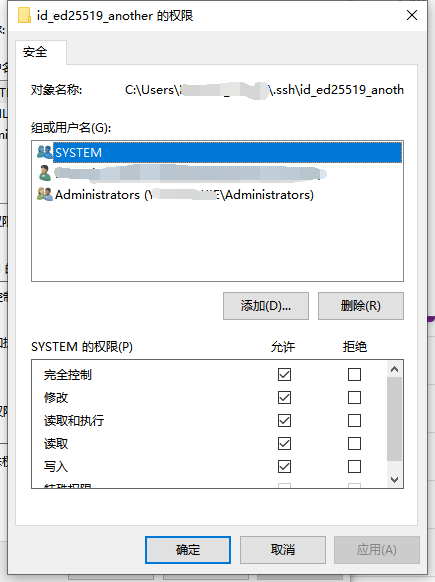
\includegraphics[width=0.7\textwidth]{figures/task1-ssh-private-key-permission-in-windows.png}
	\caption{caption:task1-ssh-private-key-permission-in-windows}
	\label{fig:task1-ssh-private-key-permission-in-windows}
\end{figure}


\begin{figure}[htbp]
	\centering
	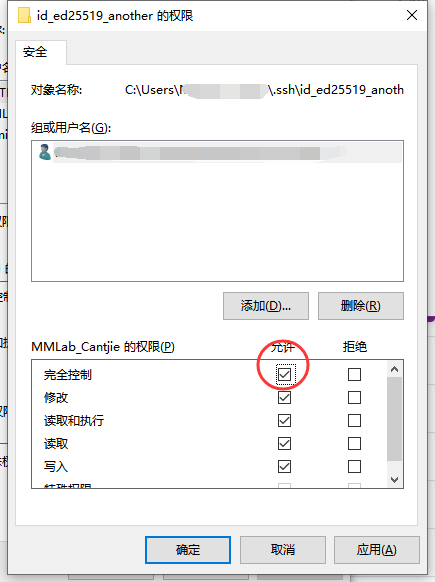
\includegraphics[width=0.7\textwidth]{figures/task1-ssh-private-key-right-permission-in-windows.png}
	\caption{caption:task1-ssh-private-key-right-permission-in-windows}
	\label{fig:task1-ssh-private-key-right-permission-in-windows}
\end{figure}